\documentclass[11pt,letterpaper]{article}
\usepackage[spanish,es-tabla]{babel}
\usepackage{fontspec}
\setmainfont{Latin Modern Roman}
\usepackage[margin=2.5cm]{geometry}
\usepackage{graphicx,booktabs,amsmath,array,hyperref,fancyhdr}

\hypersetup{colorlinks=true,linkcolor=black,urlcolor=blue}
\setlength{\parindent}{0pt}
\setlength{\parskip}{6pt}
\setlength{\emergencystretch}{3em}
\pagestyle{fancy}\fancyhf{}\fancyhead[L]{\small Comparación de bases de datos} \fancyhead[R]{\small Producción agrícola}\fancyfoot[C]{\thepage}\renewcommand{\headrulewidth}{0.3pt}\setlength{\headheight}{14pt}
\begin{document}
\begin{titlepage}\centering
{\Large\bfseries Universidad Politécnica de Chiapas\par}\vspace{0.5cm}
{\large Ingeniería en Tecnologías de la Información e Innovación Digital\par}
\vfill
{\large Actividad: Bases de datos orientadas a documentos\par}\vspace{0.9cm}
{\LARGE\bfseries Rendimiento de bases de datos documentales: caso de producción agrícola\par}\vspace{0.5cm}
{\large Comparación entre MongoDB y PostgreSQL\par}
\vfill
\begin{tabular}{rl}
Materia: & Base de datos en la nube \\
Docente: & Horacio Irán Solís Cisneros \\
Alumno: & Uzzi Yazziel Gonzaga Gómez \\
Matrícula: & 243734 \\
Fecha: & 01 de noviembre de 2026
\end{tabular}
\vspace{2cm}\end{titlepage}
\setcounter{page}{1}

\section*{Resumen}
Se compararon MongoDB y PostgreSQL JSONB con datos sintéticos de cosechas bajo tres límites de CPU y memoria. La matriz contiene 162 registros: 128 con estado \texttt{ok}, 21 con \texttt{spill}, 12 con \texttt{error} y uno con \texttt{oom}. Estos estados se conservaron tal como se registraron. Una corrida con error tiene el indicador de spill desconocido porque faltaron registros del profiler.

En Q1 con perfil A y un cliente, la mediana de las tres corridas fue 0,853 consultas por segundo para MongoDB y 0,570 para PostgreSQL. En Q2, para ese mismo perfil y concurrencia, PostgreSQL registró mayor rendimiento en las variantes medidas. Son resultados de este conjunto y configuración: no demuestran que exista un motor mejor para cualquier aplicación.

\section*{1. Equipo y entorno}
El experimento se ejecutó en un equipo con Intel Core i7-13620H, 15,64 GiB de memoria utilizable, Windows 11 y Ubuntu 24.04.3 sobre WSL2. Se utilizaron Docker Desktop 4.55.0 y Docker Engine 29.1.3. Los motores fueron MongoDB 9.0.4 y PostgreSQL 18.6; las imágenes y sus identificadores están fijados en \texttt{protocolo.json}.

Los motores se ejecutaron por separado, con datos en volúmenes de Docker. Los límites fueron: A, 4 CPU y 4096 MiB; B, 2 CPU y 2048 MiB; C, 1 CPU y 1024 MiB. El intercambio de memoria del contenedor se limitó a cero. Se usaron cAdvisor, Node Exporter y Prometheus para recopilar métricas. Las comprobaciones de infraestructura están en \texttt{resultados/\allowbreak{}verificacion\_\allowbreak{}fase1.json}.

\section*{2. Datos, consultas y método}
Se generaron 500.000 cosechas sintéticas con 1.499.983 lotes, derivados de forma determinista del conjunto inicial. Cada cosecha contiene productor, ubicación y una lista de lotes con cultivo, cajas y kilogramos por caja. El total es la suma de cajas por kilogramos por caja. El umbral de 50 kg por caja es una condición artificial del experimento, no una descripción de prácticas agrícolas reales.

Para identificar el archivo de datos se calculó una huella digital (SHA-256). Esta cadena permite comprobar si una copia conserva exactamente el mismo contenido que el archivo registrado; su valor completo se incluye en la sección de evidencia. Se verificaron 500.000 registros en cada motor y 199.729 cosechas que cumplen el filtro temporal y de estado. Esta comprobación no prueba por sí sola la igualdad exhaustiva de todos los documentos.

Q1 desanida los lotes, selecciona aquellos con más de 50 kg por caja y agrupa producción total y promedio por país y cultivo. Q2 filtra cosechas finalizadas desde el 1 de enero de 2026 y obtiene las 1.000 con mayor peso. Se evaluaron las opciones de disco de MongoDB y \texttt{work\_\allowbreak{}mem} de 4 MB y 64 MB en PostgreSQL para Q2. El conjunto expandido tiene 54 escenarios y tres repeticiones por escenario: 162 registros. La ampliación de variantes frente a las 36 celdas base del manual es una decisión del proyecto.

Cada repetición programó 60 segundos de calentamiento, 300 de medición y 60 de enfriamiento, con 1, 10 o 50 clientes. La cantidad de consultas completadas por segundo se expresa como rendimiento (QPS). Para describir los tiempos de respuesta se usan medidas que indican qué proporción de consultas terminó dentro de cierto tiempo (percentiles): el P95 deja al 95 \% de las consultas medidas en ese tiempo o menos, y el P99 deja al 99 \%. Los percentiles se calcularon con operaciones que comenzaron y terminaron dentro de la ventana; 2.991 operaciones cruzaron el cierre en el conjunto completo y no entran en esos percentiles. Esta regla puede dejar fuera consultas largas, por lo que no se deben comparar los P99 sin considerar esa limitación.

La validación funcional detallada encontró 20 grupos Q1 con sumas y conteos exactos. La mayor diferencia de promedio fue 5,23 × 10$^{-14}$ y quedó dentro de la tolerancia documentada. Las cuatro variantes Q2 produjeron los mismos 1.000 pesos en orden. El corte fue 2.719 kg y hay 998 cosechas por encima; un identificador difirió entre motores en el empate del corte. Evidencia: \texttt{resultados/\allowbreak{}validacion\_\allowbreak{}agricola\_\allowbreak{}detallada.json}. La validación de consultas no equivale a una comparación exhaustiva de todas las filas almacenadas.

El umbral de diferencia de ritmo del reloj fue menor a 2,5 \%. El límite de huecos interiores de telemetría cambió durante la matriz: 2,5 segundos para las primeras 16 corridas, 4 segundos para las siguientes 45 y 6 segundos desde el escenario 62; se mantuvo una cobertura mínima del 90 \%. Son decisiones del proyecto, no límites comprobados del profesor. Un intervalo sin muestras puede ocultar picos breves. Para diagnosticar spill se utilizó el profiler de MongoDB, cuya instrumentación añade carga. Su colección creció de 1 MiB a 256 MiB después de la corrida 82; esto puede afectar la comparación entre etapas.

\section*{3. Resultados consolidados}
El valor central de las repeticiones ordenadas (mediana) resume cada escenario. Las medianas siguientes se calculan sobre las repeticiones con estado \texttt{ok} o \texttt{spill}; los estados \texttt{error} y \texttt{oom} se mantienen en el CSV original. El resumen completo, con número de repeticiones, mínimo y máximo por escenario, está en \texttt{resultados/\allowbreak{}resumen\_\allowbreak{}agricola.csv}. Cinco escenarios tienen menos de tres repeticiones utilizables. El QPS es consultas por segundo; las latencias están en milisegundos.

\begin{center}\small\resizebox{\textwidth}{!}{\begin{tabular}{llrrr}\toprule
Perfil A, 1 cliente & Motor & Mediana QPS & Mediana P95 (ms) & Mediana P99 (ms) \\ \midrule
Q1 & MongoDB & 0,853 & 1.209,6 & 1.252,2 \\ 
Q1 & PostgreSQL & 0,570 & 1.814,4 & 1.852,9 \\ 
Q2 sin disco / 4 MB & MongoDB & 2,667 & 408,3 & 429,1 \\ 
Q2 sin disco / 4 MB & PostgreSQL & 9,870 & 111,0 & 127,0 \\ 
Q2 con disco / 64 MB & MongoDB & 2,647 & 413,5 & 431,1 \\ 
Q2 con disco / 64 MB & PostgreSQL & 9,663 & 114,4 & 124,6 \\ 
\bottomrule\end{tabular}}\end{center}
Las opciones de Q2 son tratamientos distintos, no configuraciones equivalentes entre motores. La comparación debe leerse junto con los límites y los planes, y no atribuirse a una sola causa. En Q1 con perfil A y 50 clientes, las medianas de P99 fueron 36.105,7 ms en MongoDB y 166.957,9 ms en PostgreSQL; estas cifras no eliminan la advertencia sobre operaciones que cruzaron la ventana.

En PostgreSQL Q1 con 50 clientes y perfil B se registraron dos errores y un OOM; con perfil C hubo tres errores. En MongoDB Q2 con 50 clientes y perfil C, ambas variantes registraron tres errores cada una. No hay medianas de rendimiento utilizables para esos cuatro escenarios. El quinto escenario incompleto es MongoDB A, Q2 sin disco, 10 clientes: dos \texttt{ok} y un \texttt{error} por evidencia de profiler incompleta. No se interpretó su spill desconocido como falso.

En 26 corridas con estado \texttt{ok} o \texttt{spill} hubo menos de 100 latencias completas en la ventana. En ellas el P99 es especialmente sensible a una sola observación. Los contadores OOM deben interpretarse mediante su cambio durante la ventana, no solo por un valor acumulado. El caso OOM de PostgreSQL B/Q1/50 mostró un incremento de \texttt{oom\_\allowbreak{}kill} de 1 a 2 durante la corrida.

\section*{4. Gráficas}
Las gráficas se generaron con \texttt{scripts/\allowbreak{}graficar\_\allowbreak{}agricola.py} a partir de los resultados y métricas guardadas. Para leerlas, una cifra de QPS mayor indica más consultas completadas por segundo; un tiempo de respuesta menor indica que las consultas terminan más rápido. Cada gráfica ayuda a observar un aspecto distinto:

\begin{minipage}{\textwidth}
\begin{center}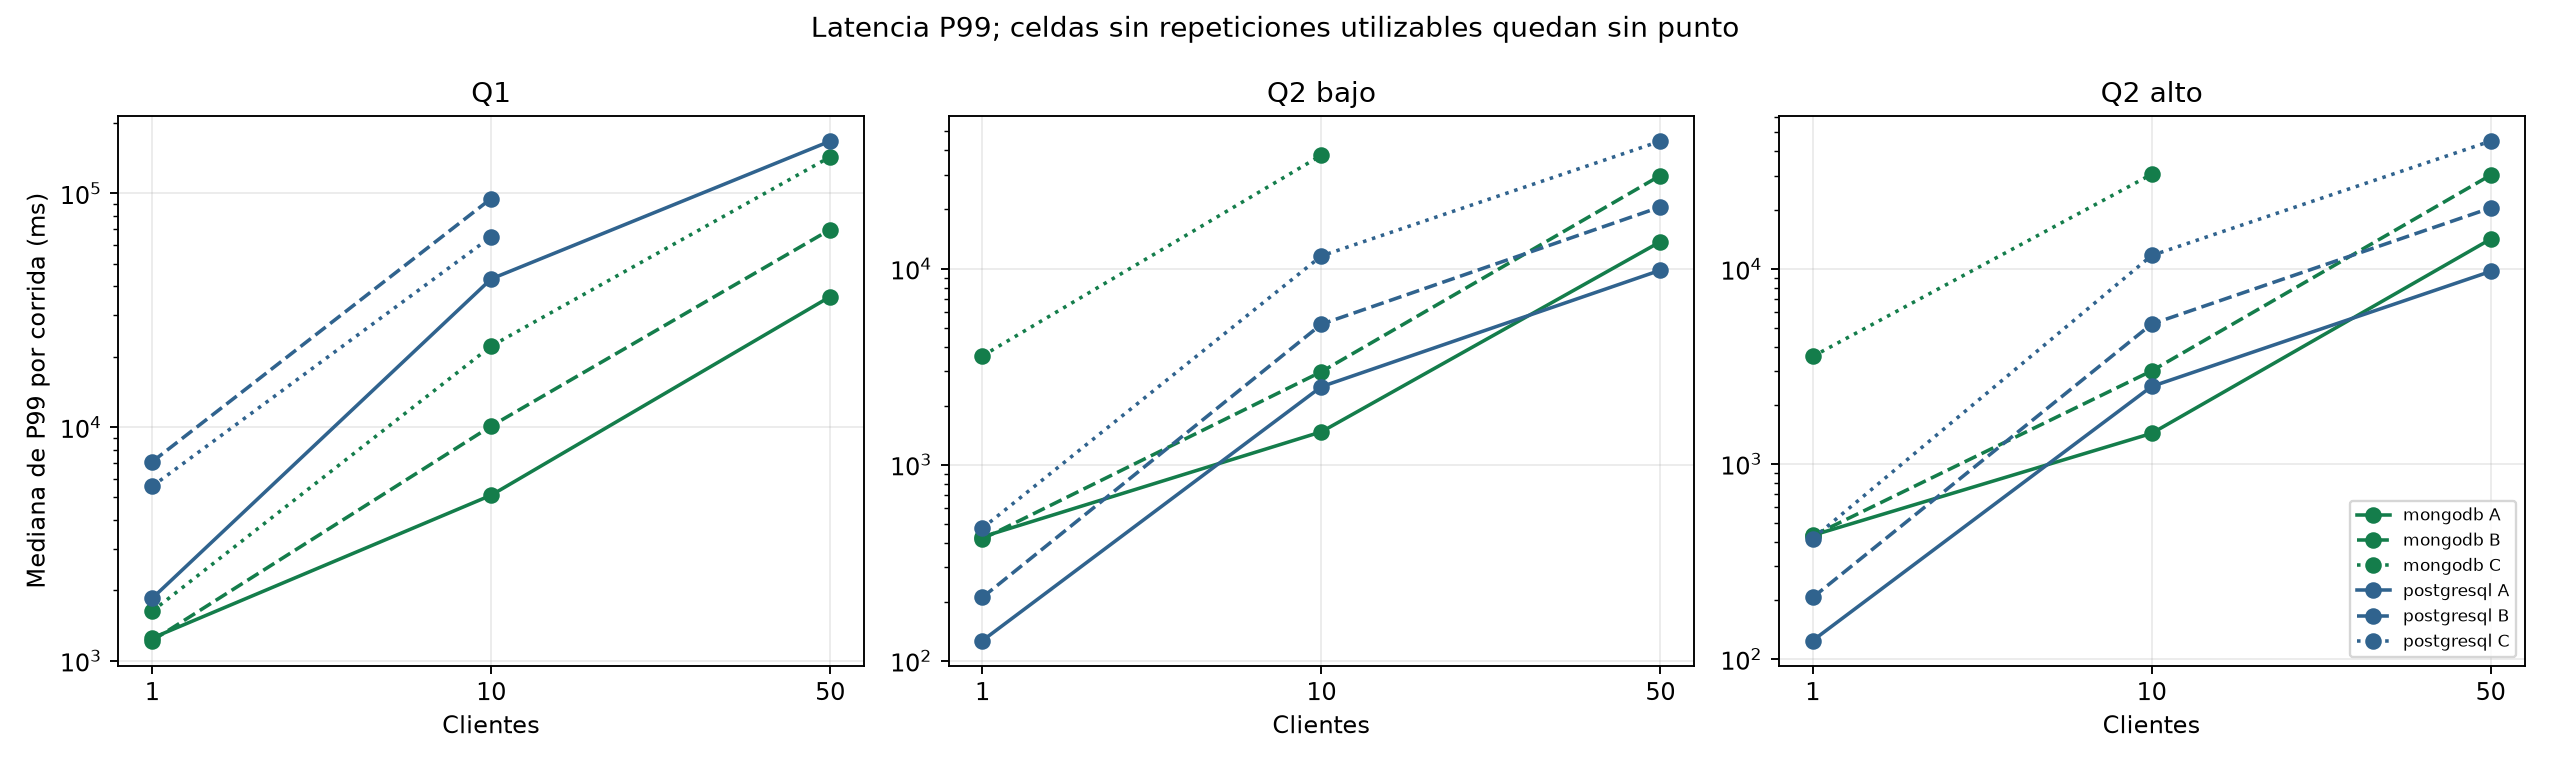
\includegraphics[width=\textwidth,height=0.68\textheight,keepaspectratio]{../resultados/graficas_agricola/p99_concurrencia.png}\par\small\textbf{Figura. Tiempo de respuesta y número de clientes}\end{center}
Mediana de P99 por escenario. La escala vertical es logarítmica y los escenarios sin repeticiones utilizables no tienen punto. Q2 bajo representa sin disco en MongoDB y 4 MB en PostgreSQL; Q2 alto representa con disco y 64 MB, respectivamente. Permite observar cómo cambia el tiempo de respuesta de las consultas más lentas al aumentar el número de clientes. En una escala logarítmica, distancias iguales representan multiplicaciones, no incrementos iguales.
\end{minipage}\par

\begin{minipage}{\textwidth}
\begin{center}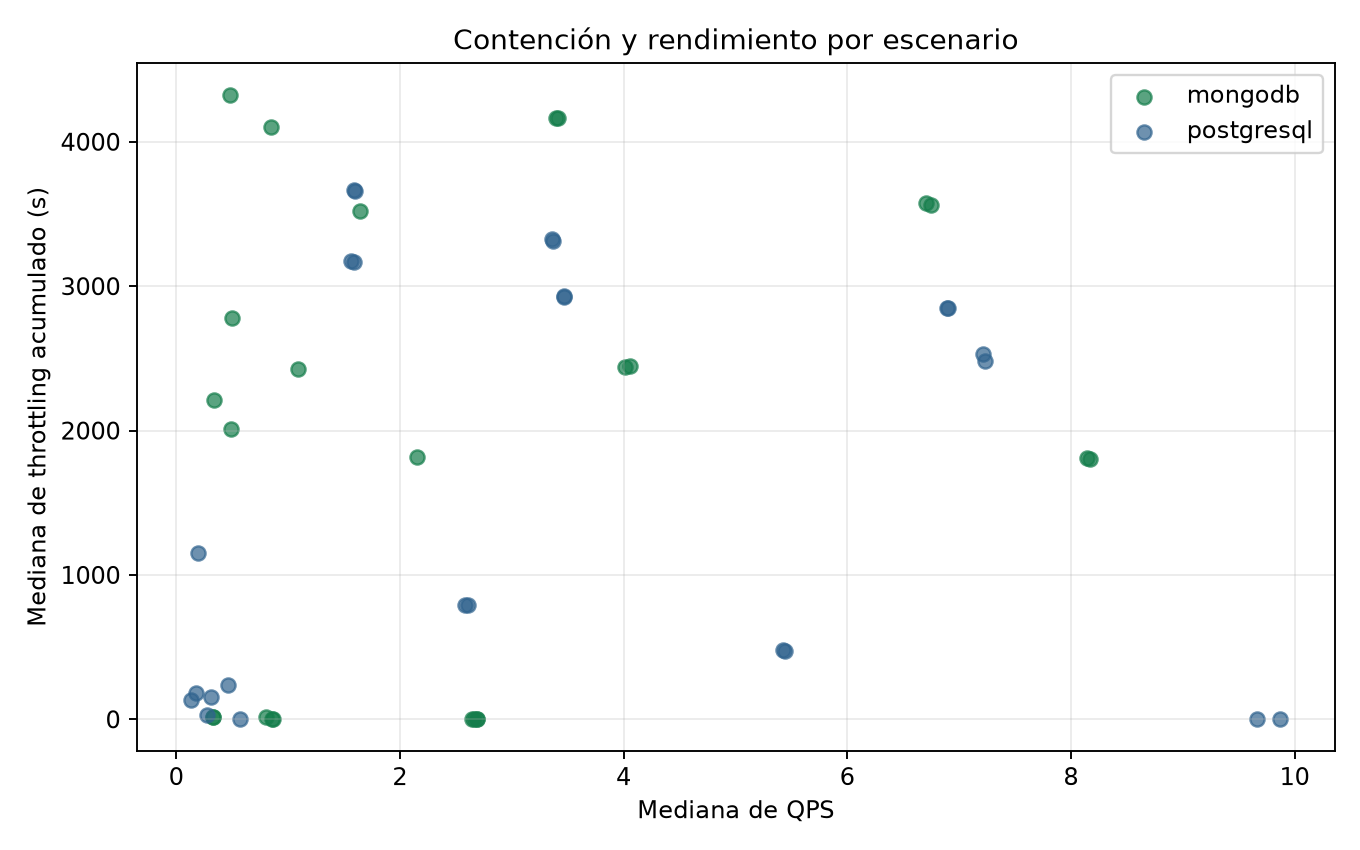
\includegraphics[width=\textwidth,height=0.68\textheight,keepaspectratio]{../resultados/graficas_agricola/throttling_qps.png}\par\small\textbf{Figura. Rendimiento y limitación del procesador}\end{center}
Relaciona las consultas completadas por segundo con el tiempo acumulado en que se limitó el uso del procesador (throttling). Ayuda a observar si ambos valores aparecen juntos en los escenarios medidos; por sí sola no demuestra que uno cause el otro.
\end{minipage}\par

\begin{minipage}{\textwidth}
\begin{center}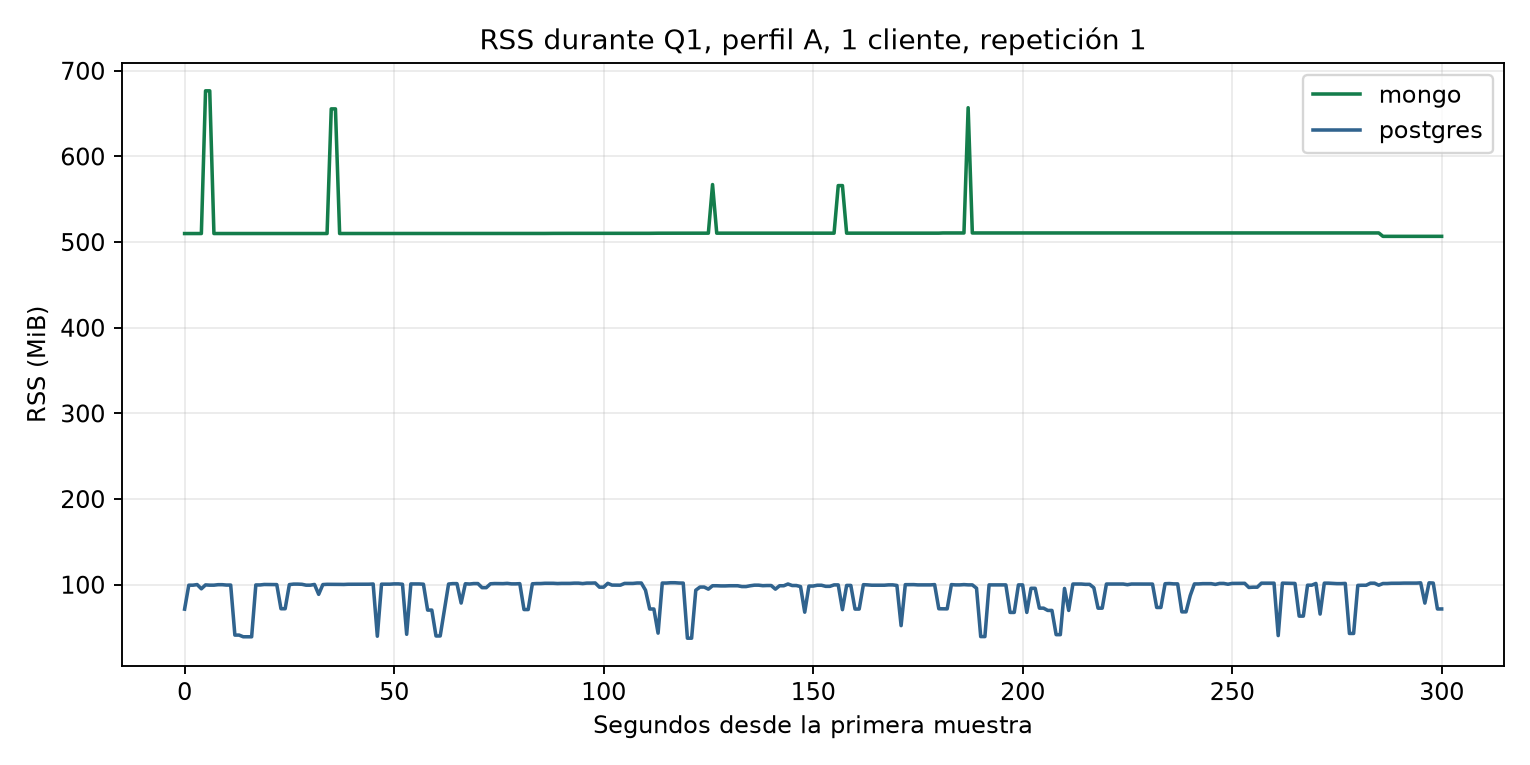
\includegraphics[width=\textwidth,height=0.68\textheight,keepaspectratio]{../resultados/graficas_agricola/rss_ejemplo.png}\par\small\textbf{Figura. Memoria residente durante una corrida}\end{center}
Muestra cómo cambia con el tiempo una medida de la memoria residente (RSS) en Q1, perfil A y un cliente, durante la primera repetición de cada motor. Las ejecuciones fueron separadas y se alinearon por tiempo relativo. El RSS mostrado no equivale al uso total de memoria.
\end{minipage}\par

\section*{5. Planes de ejecución}
Los planes de \texttt{resultados/\allowbreak{}planes\_\allowbreak{}agricola/\allowbreak{}} se obtuvieron después de la matriz, con perfil A, como validación puntual; no son mediciones de rendimiento de la matriz. En MongoDB, Q1 mostró \texttt{COLLSCAN} sobre 500.000 documentos y no reportó uso de disco en ese plan. Q2 mostró \texttt{IXSCAN} sobre fecha y examinó 249.767 documentos, con \texttt{usedDisk=false} en las dos variantes observadas.

En PostgreSQL, el plan Q1 con 4 MB mostró lectura secuencial, expansión de lotes y ordenamiento \texttt{external merge}, con bloques temporales. Los planes Q2 de 4 y 64 MB mostraron \texttt{Seq Scan} y \texttt{top-N heapsort}, sin bloques temporales en esas ejecuciones. Un plan puntual no demuestra que todas las repeticiones o cargas concurrentes se comporten igual.

\section*{6. Interpretación y limitaciones}
\textbf{M1.} En los ejemplos de Q1, el P99 aumenta al crecer la concurrencia. En MongoDB A pasó de una mediana de 1.252 ms con un cliente a 36.106 ms con 50; en PostgreSQL A pasó de 1.853 ms a 166.958 ms. Primero se calculó el P99 de cada repetición y después se tomó el valor central de esos resultados (mediana de percentiles por corrida); no es el P99 de todas las consultas juntas. Estas cifras deben leerse con sus cantidades de muestras, errores y operaciones que quedaron fuera de ventana.

\textbf{M2.} Bajo estas condiciones, PostgreSQL registró spill en las repeticiones utilizables de Q1; el plan puntual también mostró ordenamiento externo. El profiler de MongoDB no detectó spill en las corridas para las que pudo comprobarse, pero una corrida tiene spill desconocido. El OOM observado demuestra un fallo por memoria en una corrida concreta; no establece un umbral universal de producción.

\textbf{M3.} Como referencia parcial, en Q1 con perfil A y un cliente, la mediana de CPU consumida durante la ventana de 300 segundos fue 305,1 segundos de CPU en MongoDB y 406,4 en PostgreSQL; la mediana del RSS máximo fue 653,3 MiB y 102,4 MiB, respectivamente. Los segundos de CPU pueden superar el tiempo de pared cuando se usan varios núcleos. Estas cifras representan consumo del contenedor en la ventana, no por documento.

No se registró de manera fiable el número de documentos examinados en cada consulta de la matriz. Por ello no calculamos una cifra precisa de CPU o memoria por cada 1.000 documentos procesados. Los planes puntuales son evidencia útil, pero no justifican asignar su conteo a todas las repeticiones y concurrencias.

Otras limitaciones incluyen datos sintéticos simplificados, cambios de criterios de telemetría y de tamaño del profiler durante la ejecución, posible interferencia del equipo anfitrión y diferencias de instrumentación entre motores. La limpieza de caché de Linux no garantiza vaciar los buffers internos ni la caché de Windows. La medición de spill en PostgreSQL usa logs de archivos temporales en una ventana ampliada, por lo que algunos archivos cercanos a los límites pueden pertenecer al calentamiento o al cierre de consultas.

\section*{7. Recomendaciones}
Para una carga semejante a la estudiada, conviene probar ambos motores con las consultas y datos propios antes de seleccionar uno. Es importante medir también los errores y las operaciones que no terminan en la ventana, y no dimensionar recursos solo con QPS o P99 de corridas exitosas.

Para ordenar o agrupar datos, revisar planes e índices y controlar memoria por operación y concurrencia. En contenedores con poca memoria, limitar el número de clientes simultáneos puede reducir la presión, pero el valor adecuado debe medirse para cada sistema. Para futuros experimentos, registrar documentos examinados por operación, capturar resultados que cruzan el fin de ventana y fijar desde el principio los criterios de calidad y la capacidad del profiler.

\section*{Evidencia y reproducibilidad}
\begin{itemize}
\item Datos sintéticos y generación: \texttt{agricola/\allowbreak{}generar\_\allowbreak{}dataset.py}; manifiesto local \texttt{Otros/\allowbreak{}dataset\_\allowbreak{}agricola/\allowbreak{}manifiesto.json}. Huella SHA-256 del archivo agrícola: \texttt{2f73f8a70f7d59b4\allowbreak{}ef0e6f932a725000\allowbreak{}c7b7be2e0368ec77\allowbreak{}4c6358e03d2b9d1a}.
\item Consultas y validación: \texttt{agricola/\allowbreak{}} y \texttt{resultados/\allowbreak{}validacion\_\allowbreak{}agricola\_\allowbreak{}detallada.json}.
\item CSV de las 162 corridas: \texttt{resultados/\allowbreak{}matriz\_\allowbreak{}agricola.csv}; SHA-256 \texttt{68842a8d9b398386\allowbreak{}549cf26a6b89b6e8\allowbreak{}4352fc1e995858ee\allowbreak{}45b28f853ed25d33}.
\item Análisis reproducible: \texttt{scripts/\allowbreak{}analizar\_\allowbreak{}resultados.py}; resultados \texttt{resultados/\allowbreak{}analisis\_\allowbreak{}agricola.json} y \texttt{resultados/\allowbreak{}resumen\_\allowbreak{}agricola.csv}.
\item Planes agrícolas y gráficas: \texttt{resultados/\allowbreak{}planes\_\allowbreak{}agricola/\allowbreak{}} y \texttt{resultados/\allowbreak{}graficas\_\allowbreak{}agricola/\allowbreak{}}.
\item Evidencia cruda, intentos descartados y bitácora: \texttt{Otros/\allowbreak{}} y \texttt{contexto/\allowbreak{}}, guardados localmente y excluidos de Git.
\end{itemize}
\section*{Referencias}
\begin{itemize}
\item Manuales de la actividad: \texttt{playbook.pdf} y \texttt{playbook\_\allowbreak{}sesion.pdf}, proporcionados para el experimento.
\item MongoDB, \href{https://www.mongodb.com/docs/manual/tutorial/manage-the-database-profiler/}{Database Profiler}: funcionamiento y sobrecarga del profiler.
\item PostgreSQL, \href{https://www.postgresql.org/docs/current/using-explain.html}{Using EXPLAIN}: interpretación de planes y buffers.
\item Prometheus, \href{https://prometheus.io/docs/prometheus/latest/querying/basics/}{Querying basics}: consultas y vectores de rango.
\end{itemize}
\end{document}
